\documentclass[table]{beamer}\usepackage[]{graphicx}\usepackage[]{color}
%% maxwidth is the original width if it is less than linewidth
%% otherwise use linewidth (to make sure the graphics do not exceed the margin)
\makeatletter
\def\maxwidth{ %
  \ifdim\Gin@nat@width>\linewidth
    \linewidth
  \else
    \Gin@nat@width
  \fi
}
\makeatother

\definecolor{fgcolor}{rgb}{0.345, 0.345, 0.345}
\newcommand{\hlnum}[1]{\textcolor[rgb]{0.686,0.059,0.569}{#1}}%
\newcommand{\hlstr}[1]{\textcolor[rgb]{0.192,0.494,0.8}{#1}}%
\newcommand{\hlcom}[1]{\textcolor[rgb]{0.678,0.584,0.686}{\textit{#1}}}%
\newcommand{\hlopt}[1]{\textcolor[rgb]{0,0,0}{#1}}%
\newcommand{\hlstd}[1]{\textcolor[rgb]{0.345,0.345,0.345}{#1}}%
\newcommand{\hlkwa}[1]{\textcolor[rgb]{0.161,0.373,0.58}{\textbf{#1}}}%
\newcommand{\hlkwb}[1]{\textcolor[rgb]{0.69,0.353,0.396}{#1}}%
\newcommand{\hlkwc}[1]{\textcolor[rgb]{0.333,0.667,0.333}{#1}}%
\newcommand{\hlkwd}[1]{\textcolor[rgb]{0.737,0.353,0.396}{\textbf{#1}}}%
\let\hlipl\hlkwb

\usepackage{framed}
\makeatletter
\newenvironment{kframe}{%
 \def\at@end@of@kframe{}%
 \ifinner\ifhmode%
  \def\at@end@of@kframe{\end{minipage}}%
  \begin{minipage}{\columnwidth}%
 \fi\fi%
 \def\FrameCommand##1{\hskip\@totalleftmargin \hskip-\fboxsep
 \colorbox{shadecolor}{##1}\hskip-\fboxsep
     % There is no \\@totalrightmargin, so:
     \hskip-\linewidth \hskip-\@totalleftmargin \hskip\columnwidth}%
 \MakeFramed {\advance\hsize-\width
   \@totalleftmargin\z@ \linewidth\hsize
   \@setminipage}}%
 {\par\unskip\endMakeFramed%
 \at@end@of@kframe}
\makeatother

\definecolor{shadecolor}{rgb}{.97, .97, .97}
\definecolor{messagecolor}{rgb}{0, 0, 0}
\definecolor{warningcolor}{rgb}{1, 0, 1}
\definecolor{errorcolor}{rgb}{1, 0, 0}
\newenvironment{knitrout}{}{} % an empty environment to be redefined in TeX

\usepackage{alltt}

%\setbeamertemplate{background}{\includegraphics[width=\paperwidth,height=\paperheight,keepaspectratio]{ages_background2.png}}

\usepackage[ngerman,english]{babel}
\usepackage{lmodern} % schrift besser lesbar
\usepackage[T1]{fontenc}
\usepackage[utf8]{inputenc}
\usepackage{comment}

\usepackage{amsmath, amsthm}
\usepackage{amssymb}
\usepackage{bbm} % "Blackboard-style" cm fonts
\usepackage{xcolor}
\usepackage{colortbl}

\usepackage[backend = bibtex, natbib = true, style = numeric, sorting = none, citestyle = authoryear]{biblatex}
\addbibresource{../../diss_tex/references/mybib.bib}

\usetheme{Boadilla}

%\definecolor{ages}{RGB}{204,164,0}
%\usecolortheme[named=ages]{structure}

\setbeamertemplate{blocks}[rounded][shadow=false]
% \setbeamercolor{frametitle}{bg=structure.fg!20!bg}
\setbeamercovered{transparent}
\beamertemplatenavigationsymbolsempty
\setbeamertemplate{footline}[frame number]

\newcommand\numbered{\setbeamertemplate{footline}[frame number]}
\newcommand\unnumbered{\setbeamertemplate{footline}{}}


\newcommand{\Sin}[1]{\sin\left(#1\right)}%
\newcommand{\Cos}[1]{\cos\left(#1\right)}%
\newcommand{\Log}[1]{\log\left(#1\right)}%
\newcommand{\mli}[1]{\mathit{#1}}% MulitLetterIdentifier - produces nice names for multi character variables in math environments

% generate block with different colour
\newenvironment{variableblock}[3]{%
  \setbeamercolor{block body}{#2}
  \setbeamercolor{block title}{#3}
  \begin{block}{#1}}{\end{block}}
\IfFileExists{upquote.sty}{\usepackage{upquote}}{}
\begin{document}
\graphicspath{{figures/}}
%\graphicspath{{../../chapters/figures/IPD/}, {../../chapters/figures/}}
%\graphicspath{{D:/diss/chapters/figures/IPD/}} %{{paste0(getwd(), "/chapters/figures/IPD/")}} %{../figures/IPD/}
%% initialize %%



%%%%
\title{Modelling in Public Health}
\subtitle{SE Scientific Communication, 2019}
\author{Lukas Richter}
\date[]{28. June 2019}

% \titlegraphic{
%   
\includegraphics[width=2.0cm]{logo_ages}\hspace*{3cm}~%
%   
\includegraphics[width=2.0cm]{logo_tugraz}
% }

%10-15 min presentation


%%%%%%%%%%%%%%%%%%%%%%%%%%%%%%%%%%%%%%%%%%%%%%
{\unnumbered
\begin{frame}[noframenumbering]
  \titlepage
\end{frame}}
%%%%%%%%%%%%%%%%%%%%%%%%%%%%%%%%%%%%%%%%%%%%%%

%%%%%%%%%%%%%%%%%%%%%%%%%%%%%%%%%%%%%%%%%%%%%%
{\unnumbered
\begin{frame}[noframenumbering]{Content}
  \tableofcontents
\end{frame}}
%%%%%%%%%%%%%%%%%%%%%%%%%%%%%%%%%%%%%%%%%%%%%%

\section{Background}
%%%%%%%%%%%%%%%%%%%%%%%%%%%%%%%%%%%%%%%%%%%%%%
\begin{frame}[fragile]{Background}

Infectious diseases are a serious \textbf{burden} for human health \\
\vspace{0.3cm}
Results in \textbf{loss of QUALYs} and also money \\ % quality-adjusted life year
\vspace{0.3cm}
WHO: \textbf{50,000 deaths per day} due to infectious diseases \\ % many are preventable (vaccines) or curable
\vspace{0.3cm}
Outbreaks vs endemic infection \\ % infection is constantly maintained at a baseline level in a geographic area without external inputs (steady state)
\vspace{0.3cm}
Different chains \textbf{transmission}:
\begin{figure}
  \flushleft
  % \caption{Example of outbreak analytics workflow.}
  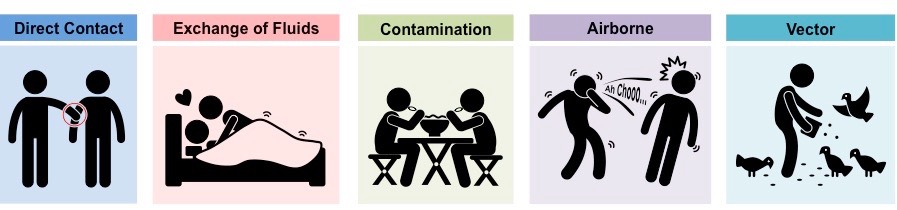
\includegraphics[width=0.85\textwidth,keepaspectratio]{disease-transmission_med.jpeg}
\end{figure}

\end{frame}
%%%%%%%%%%%%%%%%%%%%%%%%%%%%%%%%%%%%%%%%%%%%%%

%%%%%%%%%%%%%%%%%%%%%%%%%%%%%%%%%%%%%%%%%%%%%%
{
\usebackgroundtemplate{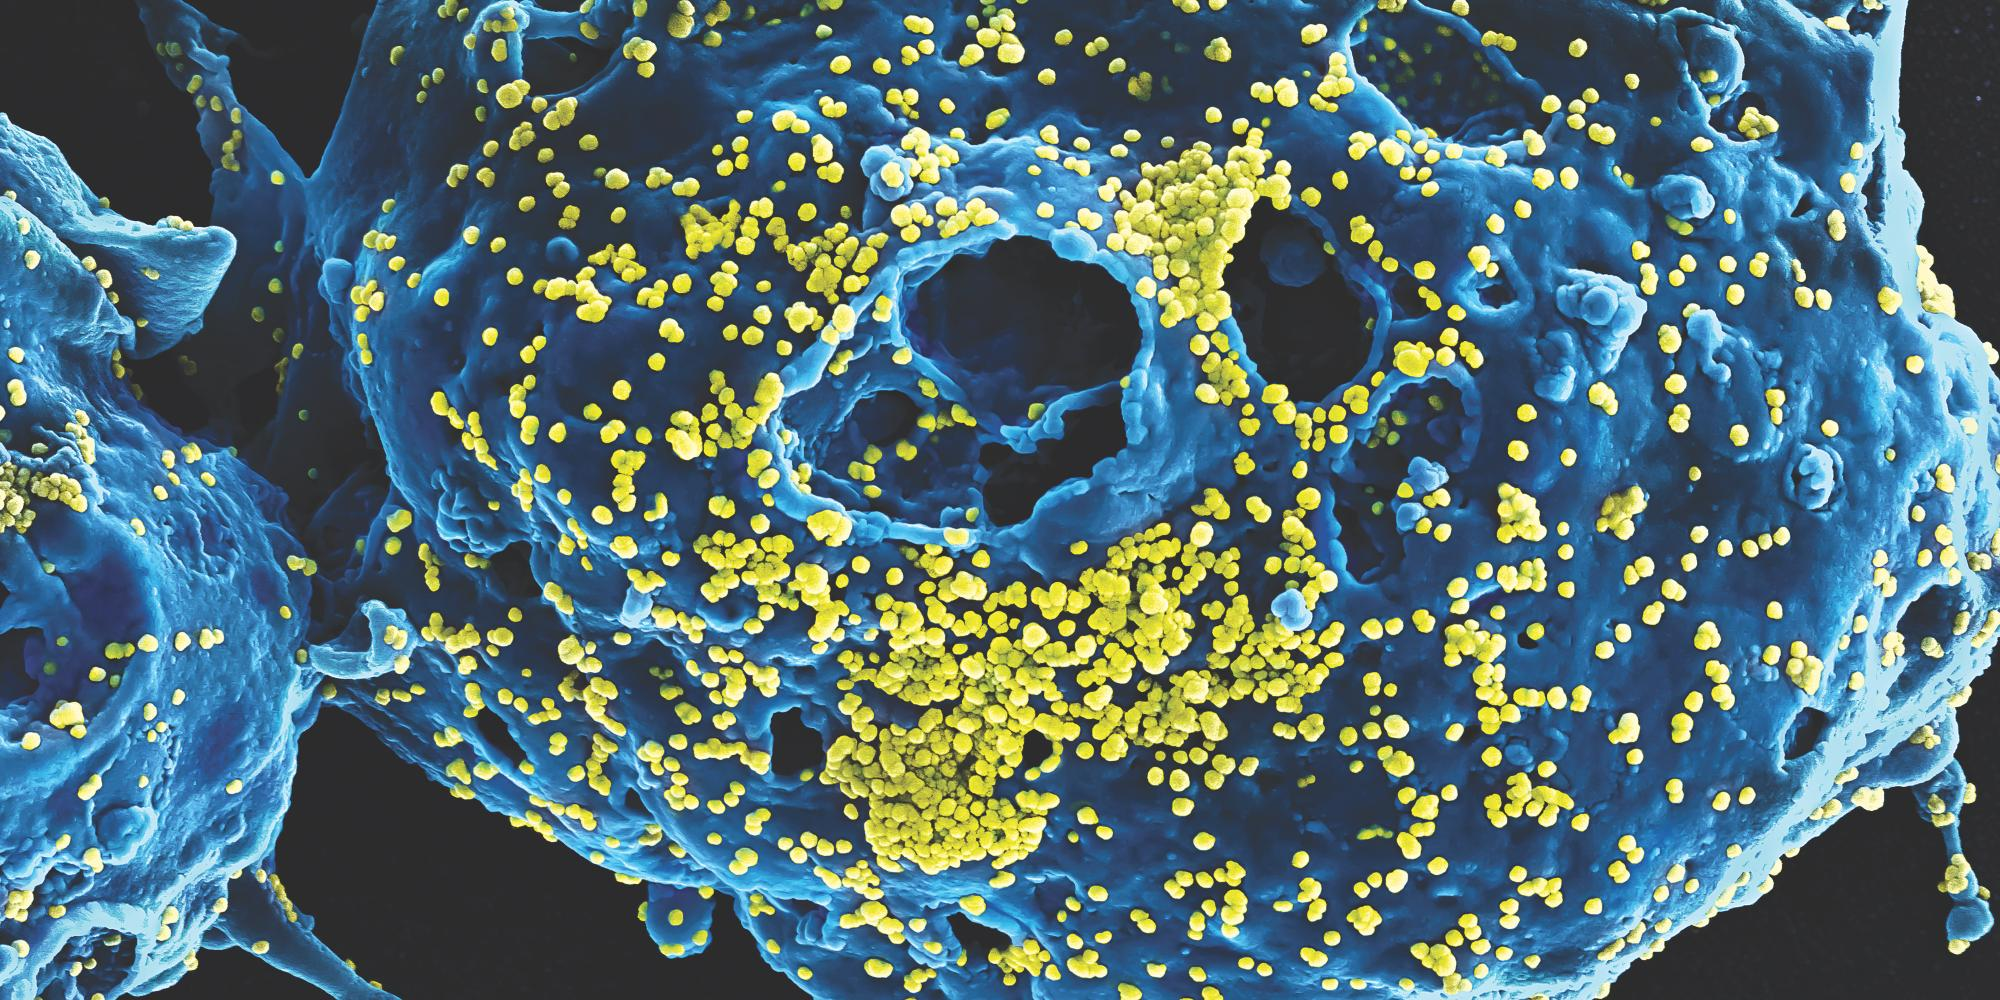
\includegraphics[height=\paperheight]{outbreak.jpg}}%
\setbeamercolor{frametitle}{bg=structure.fg!20!bg}%
\begin{frame}[fragile]{Outbreaks}

\begin{block} {Influenza pandemic ``swine flu''}
Global, 2009-2010, 100,000 -- 400,000 deaths
\end{block}
\begin{block} {Ebola}
% MERS-Cov (Middle-East Respiratory Syndrome) \\
West Africa, 2014-2016, 11,000 deaths \\
DRC, since 2018, 1,900 deaths
\end{block}
\begin{block} {Zika Virus}
Brazil, 2015-2016, ca. 215,000 cases (CHECK!) wolrdwide
\end{block}
\begin{block} {Measles}
Europe, 2019, ca. 6,300 cases from Jan--Apr \\ % Romania, Lithuania, Italy, Poland, Bulgaria, Czech Republic, France, Greece, Slovakia
Austria, 2019, more than 130 cases up to this week
\end{block}

\end{frame}
}
%%%%%%%%%%%%%%%%%%%%%%%%%%%%%%%%%%%%%%%%%%%%%%

%%%%%%%%%%%%%%%%%%%%%%%%%%%%%%%%%%%%%%%%%%%%%%
\begin{frame}[fragile]{How can modellers help?}

% \textbf{How can modellers help?} \\
% \vspace{0.3cm}
Outbreak situations: \\
\vspace{0.1cm}
\hspace{0.5cm} Exploit all data \\
\vspace{0.1cm}
\hspace{0.5cm} Inform response team in real time \\
\vspace{0.3cm}

Non outbreak situations: \\
\vspace{0.1cm}
\hspace{0.5cm} Evaluate health programmes (vaccination, WHO elimination targets) \\ % HIV-AIDS, Hepatitis C
\vspace{0.1cm}
\hspace{0.5cm} Find high impact and cost-effective interventions \\
\vspace{0.1cm}
\hspace{0.5cm} Allow evidence based decisions \\
\vspace{0.3cm}

Benefits of modelling: \\
\vspace{0.1cm}
\hspace{0.5cm} Cheap: Clinical trials are expensive and seldom large enough \\
\vspace{0.1cm}
\hspace{0.5cm} Often little or no data to analyse (new emerging diseases) \\ % WHO: At least 30 new diseases have emerged in the last 20 years
\vspace{0.3cm}

% mathematical models can help to assess potential threats and impacts early in the process, and later aid in interpreting data from complex and multifactorial systems

% The World Health Organisation's definition of public health refers to all organized measures to prevent disease, promote health, and prolong life among the population as a whole (World Health Organization, 2014). Mathematical modelling plays an increasingly important role in helping to guide the most high impact and cost-effective means of achieving these goals. Public health programmes are usually implemented over a long period of time with broad benefits to many in the community. Clinical trials are seldom large enough to capture these effects. Observational data may be used to evaluate a programme after it is underway, but have limited value in helping to predict the future impact of a proposed policy. Furthermore, public health practitioners are often required to respond to new threats, for which there is little or no previous data on which to assess the threat. Computational and mathematical models can help to assess potential threats and impacts early in the process, and later aid in interpreting data from complex and multifactorial systems. As such, these models can be critical tools in guiding public health action. However, there are a number of challenges in achieving a successful interface between modelling and public health. Here, we discuss some of these challenges.

\end{frame}
%%%%%%%%%%%%%%%%%%%%%%%%%%%%%%%%%%%%%%%%%%%%%%

%%%%%%%%%%%%%%%%%%%%%%%%%%%%%%%%%%%%%%%%%%%%%%
\begin{frame}[fragile]{Types of models}

\begin{block}{Statistical}
\begin{minipage}{.49\textwidth}
\begin{figure}
  \flushleft
  % \caption{Example of outbreak analytics workflow.}
  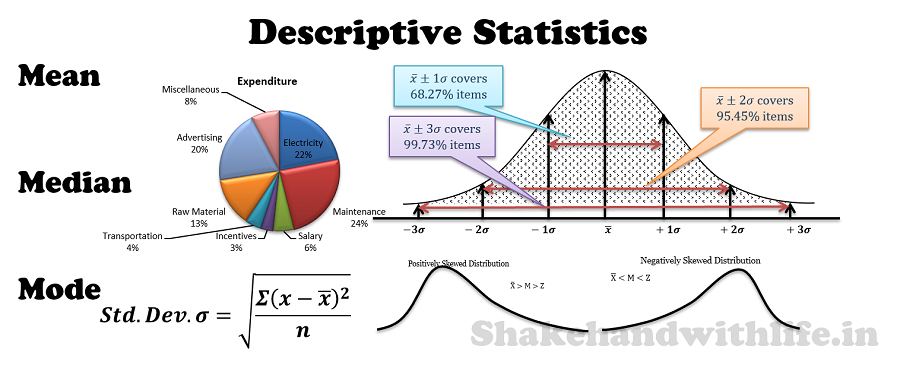
\includegraphics[width=0.9\textwidth,keepaspectratio]{statistics2.png}
\end{figure}
\end{minipage}
%%%%%%%%%%
\begin{minipage}{.49\textwidth}
Descriptive \par
\vspace{0.1cm}
Regression \par
\vspace{0.1cm}
Bayesian statistics \par
\vspace{0.1cm}
Spatial models
\end{minipage} \hfill
\end{block}
%%%%%%%%%%%%%%%%%%%%
\begin{block}{Mathematical}
\begin{minipage}{.49\textwidth}
\begin{figure}
  \flushleft
  % \caption{Example of outbreak analytics workflow.}
  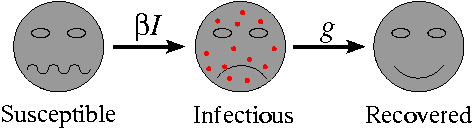
\includegraphics[width=0.9\textwidth,keepaspectratio]{sir2.png}
\end{figure}
\end{minipage} \hfill %\par\vspace{0.5cm}
%%%%%%%%%%
\begin{minipage}{.49\textwidth}
Dynamic, compartmental (SIR) \par %  origin is in the early 20th century
\vspace{0.1cm}
Stochastic - Markov chain \par
\vspace{0.1cm}
Deterministic \par
\vspace{0.1cm}
Agent-based
\end{minipage}
\end{block}
%%%%%%%%%%%%%%%%%%%%

% \vspace{1cm}
% -> visualise outcome / communication
\end{frame}
%%%%%%%%%%%%%%%%%%%%%%%%%%%%%%%%%%%%%%%%%%%%%%


% %%%%%%%%%%%%%%%%%%%%%%%%%%%%%%%%%%%%%%%%%%%%%%
% \begin{frame}[fragile]{Example of outbreak analytics workflow.}
% \begin{center}
% \begin{figure}
%   \centering
%   % \caption{Example of outbreak analytics workflow.}
%   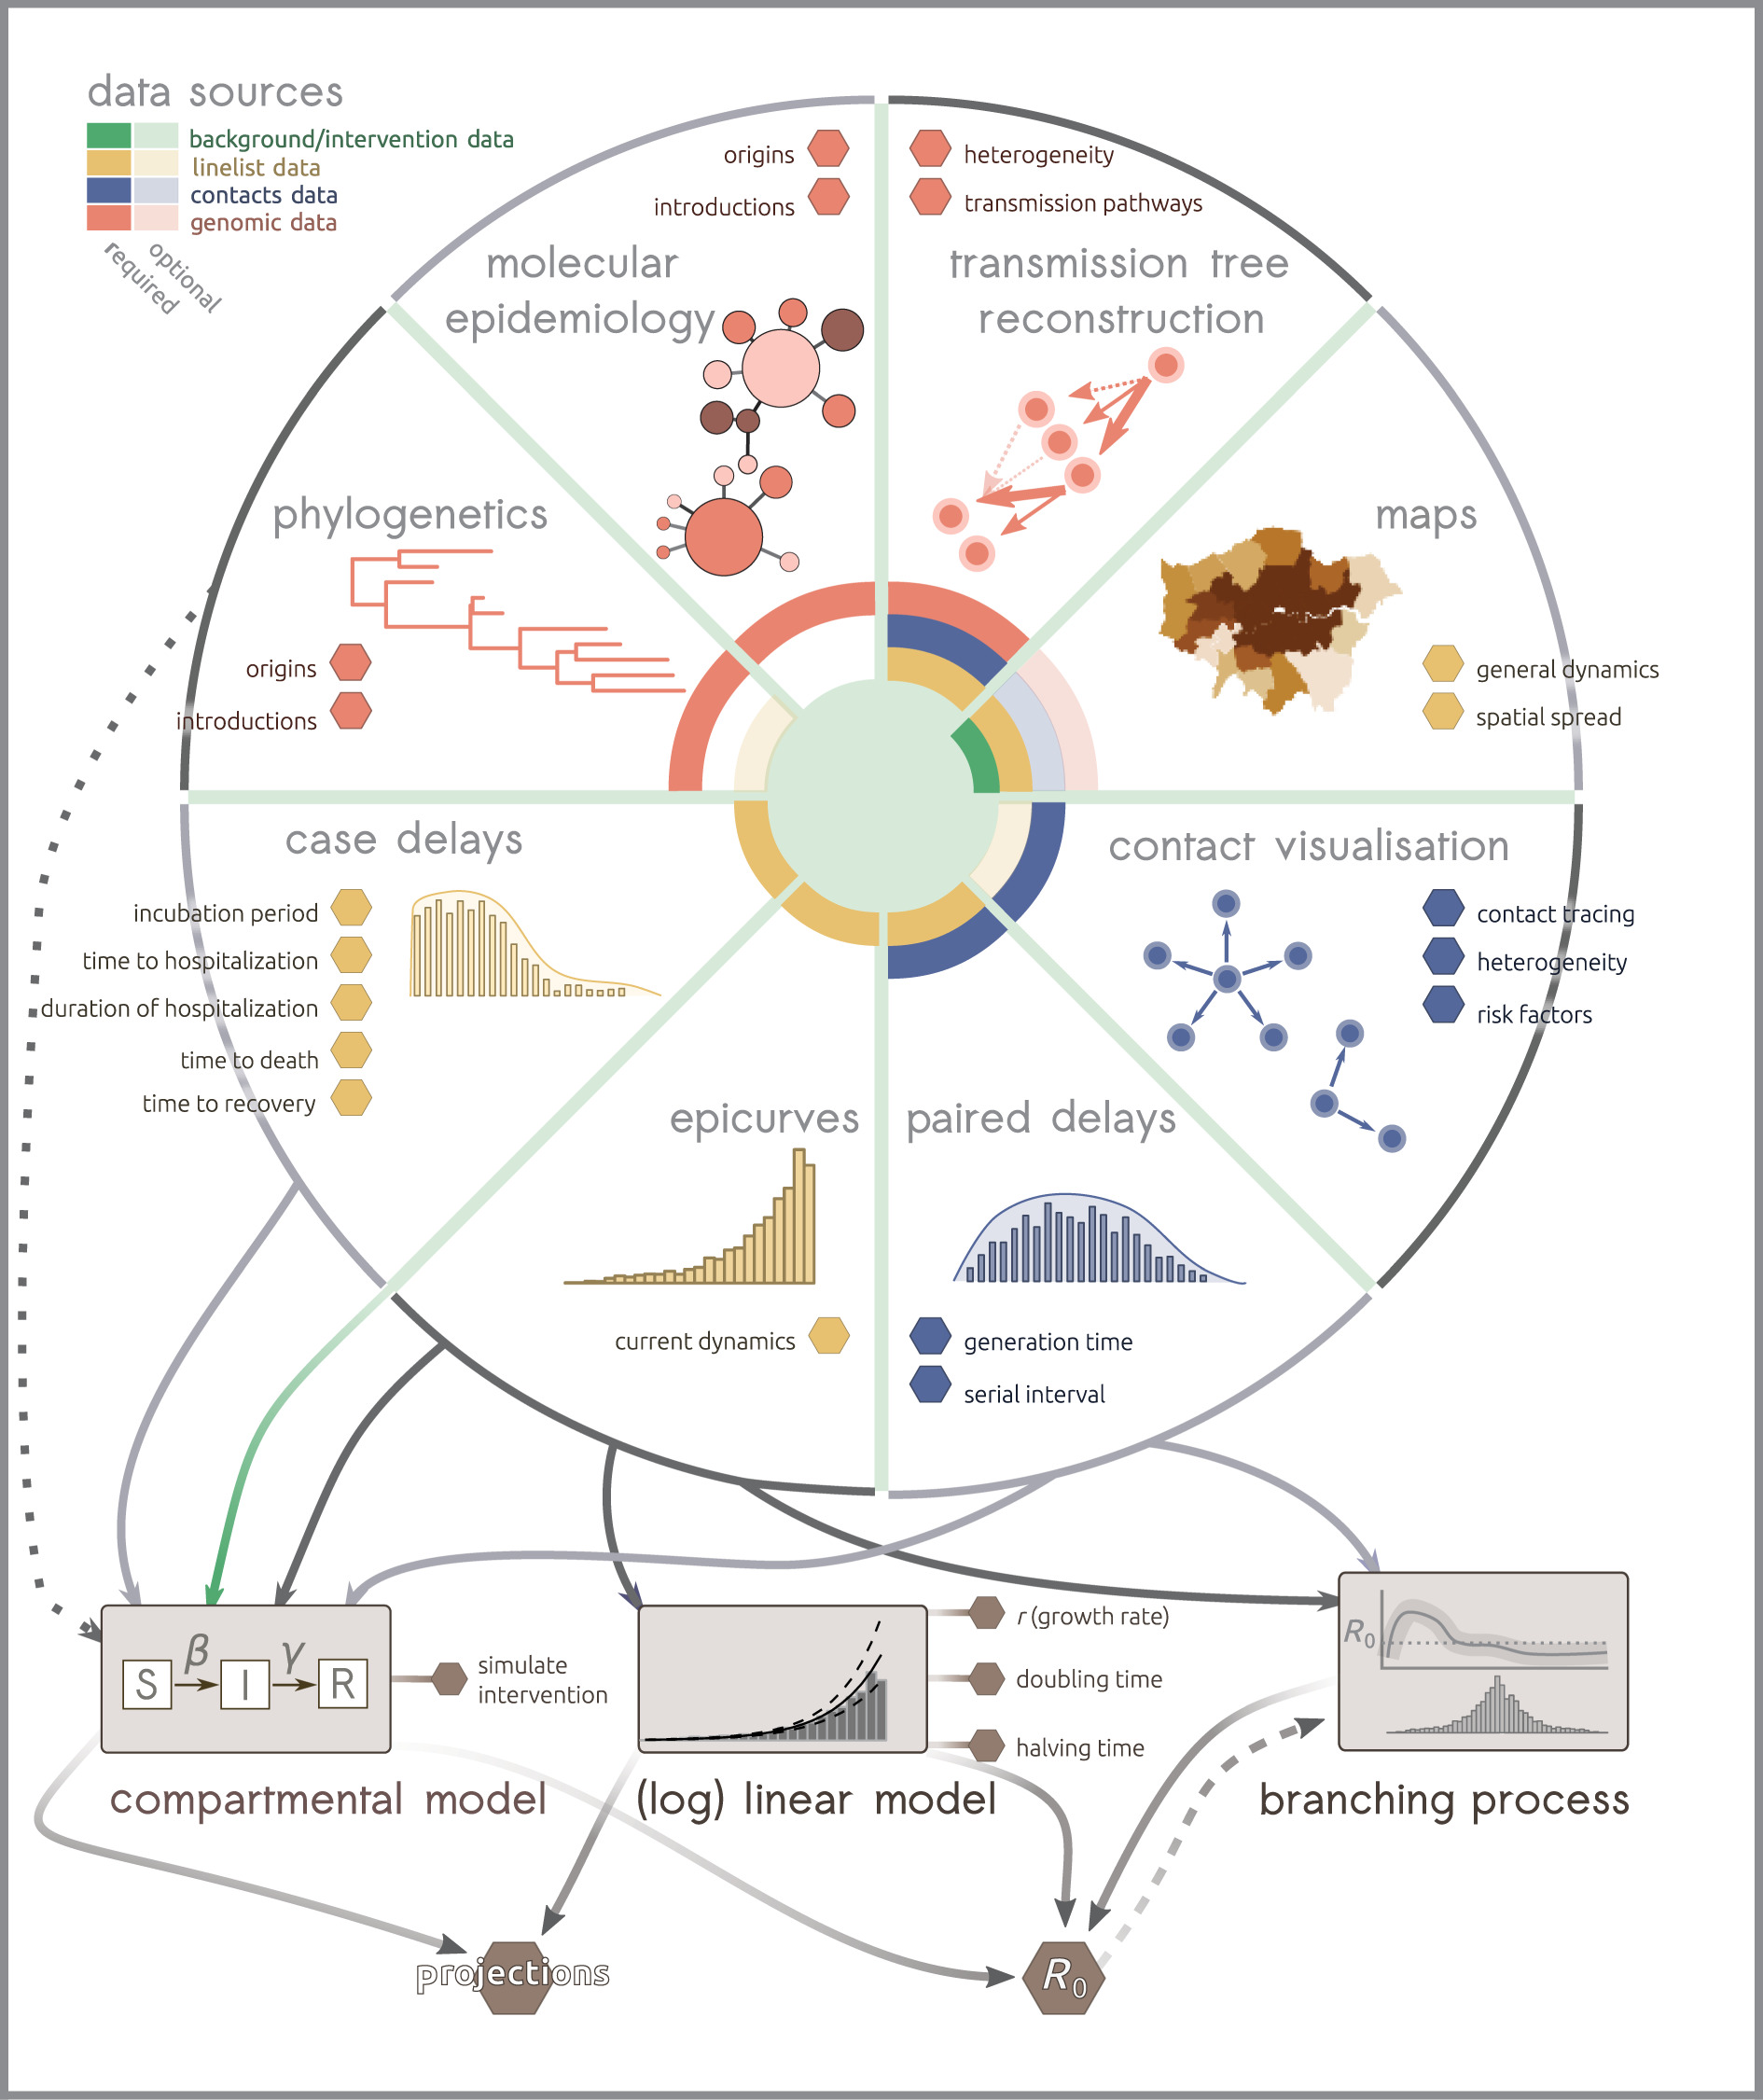
\includegraphics[width=\textwidth,height=0.8\textheight,keepaspectratio]{polonsky2019_Fig2.png}
% \end{figure}
% \end{center}
% \end{frame}
% %%%%%%%%%%%%%%%%%%%%%%%%%%%%%%%%%%%%%%%%%%%%%%

\section{Statistical models}
%%%%%%%%%%%%%%%%%%%%%%%%%%%%%%%%%%%%%%%%%%%%%%
\begin{frame}[fragile]{Intervention effect - Invasive Pneumococcal Disease (IPD)}


  Streptococcus pneumoniae-related infections:\\
  among children main cause of

    meningitis
    bacterial pneumonia
    sepsis

  90 distinct pneumococcal serotypes
  Only a small number account for invasive pneumococcal disease (IPD)
  January 2012: pneumococcal conjugate vaccine introduced in the national childhood immunisation program:

    covering 10 serotypes (PCV10)
    administered at 3rd, 5th and 12th month of life
    unded
 
  Other vaccines: PCV13, PPV23



\end{frame}
%%%%%%%%%%%%%%%%%%%%%%%%%%%%%%%%%%%%%%%%%%%%%%

%%%%%%%%%%%%%%%%%%%%%%%%%%%%%%%%%%%%%%%%%%%%%%
\begin{frame}[fragile]{IPD - The Model}
\begin{block}{Serfling-like Model}
\begin{align*}
\begin{split}
\Log{Y_t}\, =
  &\, \beta_0+\beta_1\,t + \beta_2\,\Sin{\frac{2 \pi t}{12}} + \beta_3\,\Cos{\frac{2 \pi t}{12}} \\
  &+ \beta_5\left(t-t_0\right)^+ + \mathbbm{1}_{t-t_0>0} \left[\beta_4 + \beta_6\,\sin\left(\frac{2 \pi t}{12}\right) + \beta_7\,\cos\left(\frac{2 \pi t}{12}\right)\right] \\
  &+ \Log{\mli{pop}_t}
\end{split}
\end{align*}

with
\begin{align*} 
(x)^+ = 
\begin{cases}
x, &\text{if $x > 0$,}\\
0, &\text{otherwise.}
\end{cases}
\end{align*}
\end{block}
\vfill
{\scriptsize \cite{richter2019}}
\end{frame}
%%%%%%%%%%%%%%%%%%%%%%%%%%%%%%%%%%%%%%%%%%%%%%

%%%%%%%%%%%%%%%%%%%%%%%%%%%%%%%%%%%%%%%%%%%%%%
\begin{frame}[fragile]{IPD - Results}
\begin{center}
\begin{figure}
  \centering
  \caption{Monthly incidence of (A) PCV10 ST-IPD and (B) non-PCV10 ex ST 6A-/19A-IPD, among the $\ge$50 years old, observed and modelled by a segmented negative binominal regression, Austria, January 2009-February 2017, shown are overall and seasonal trends.}
  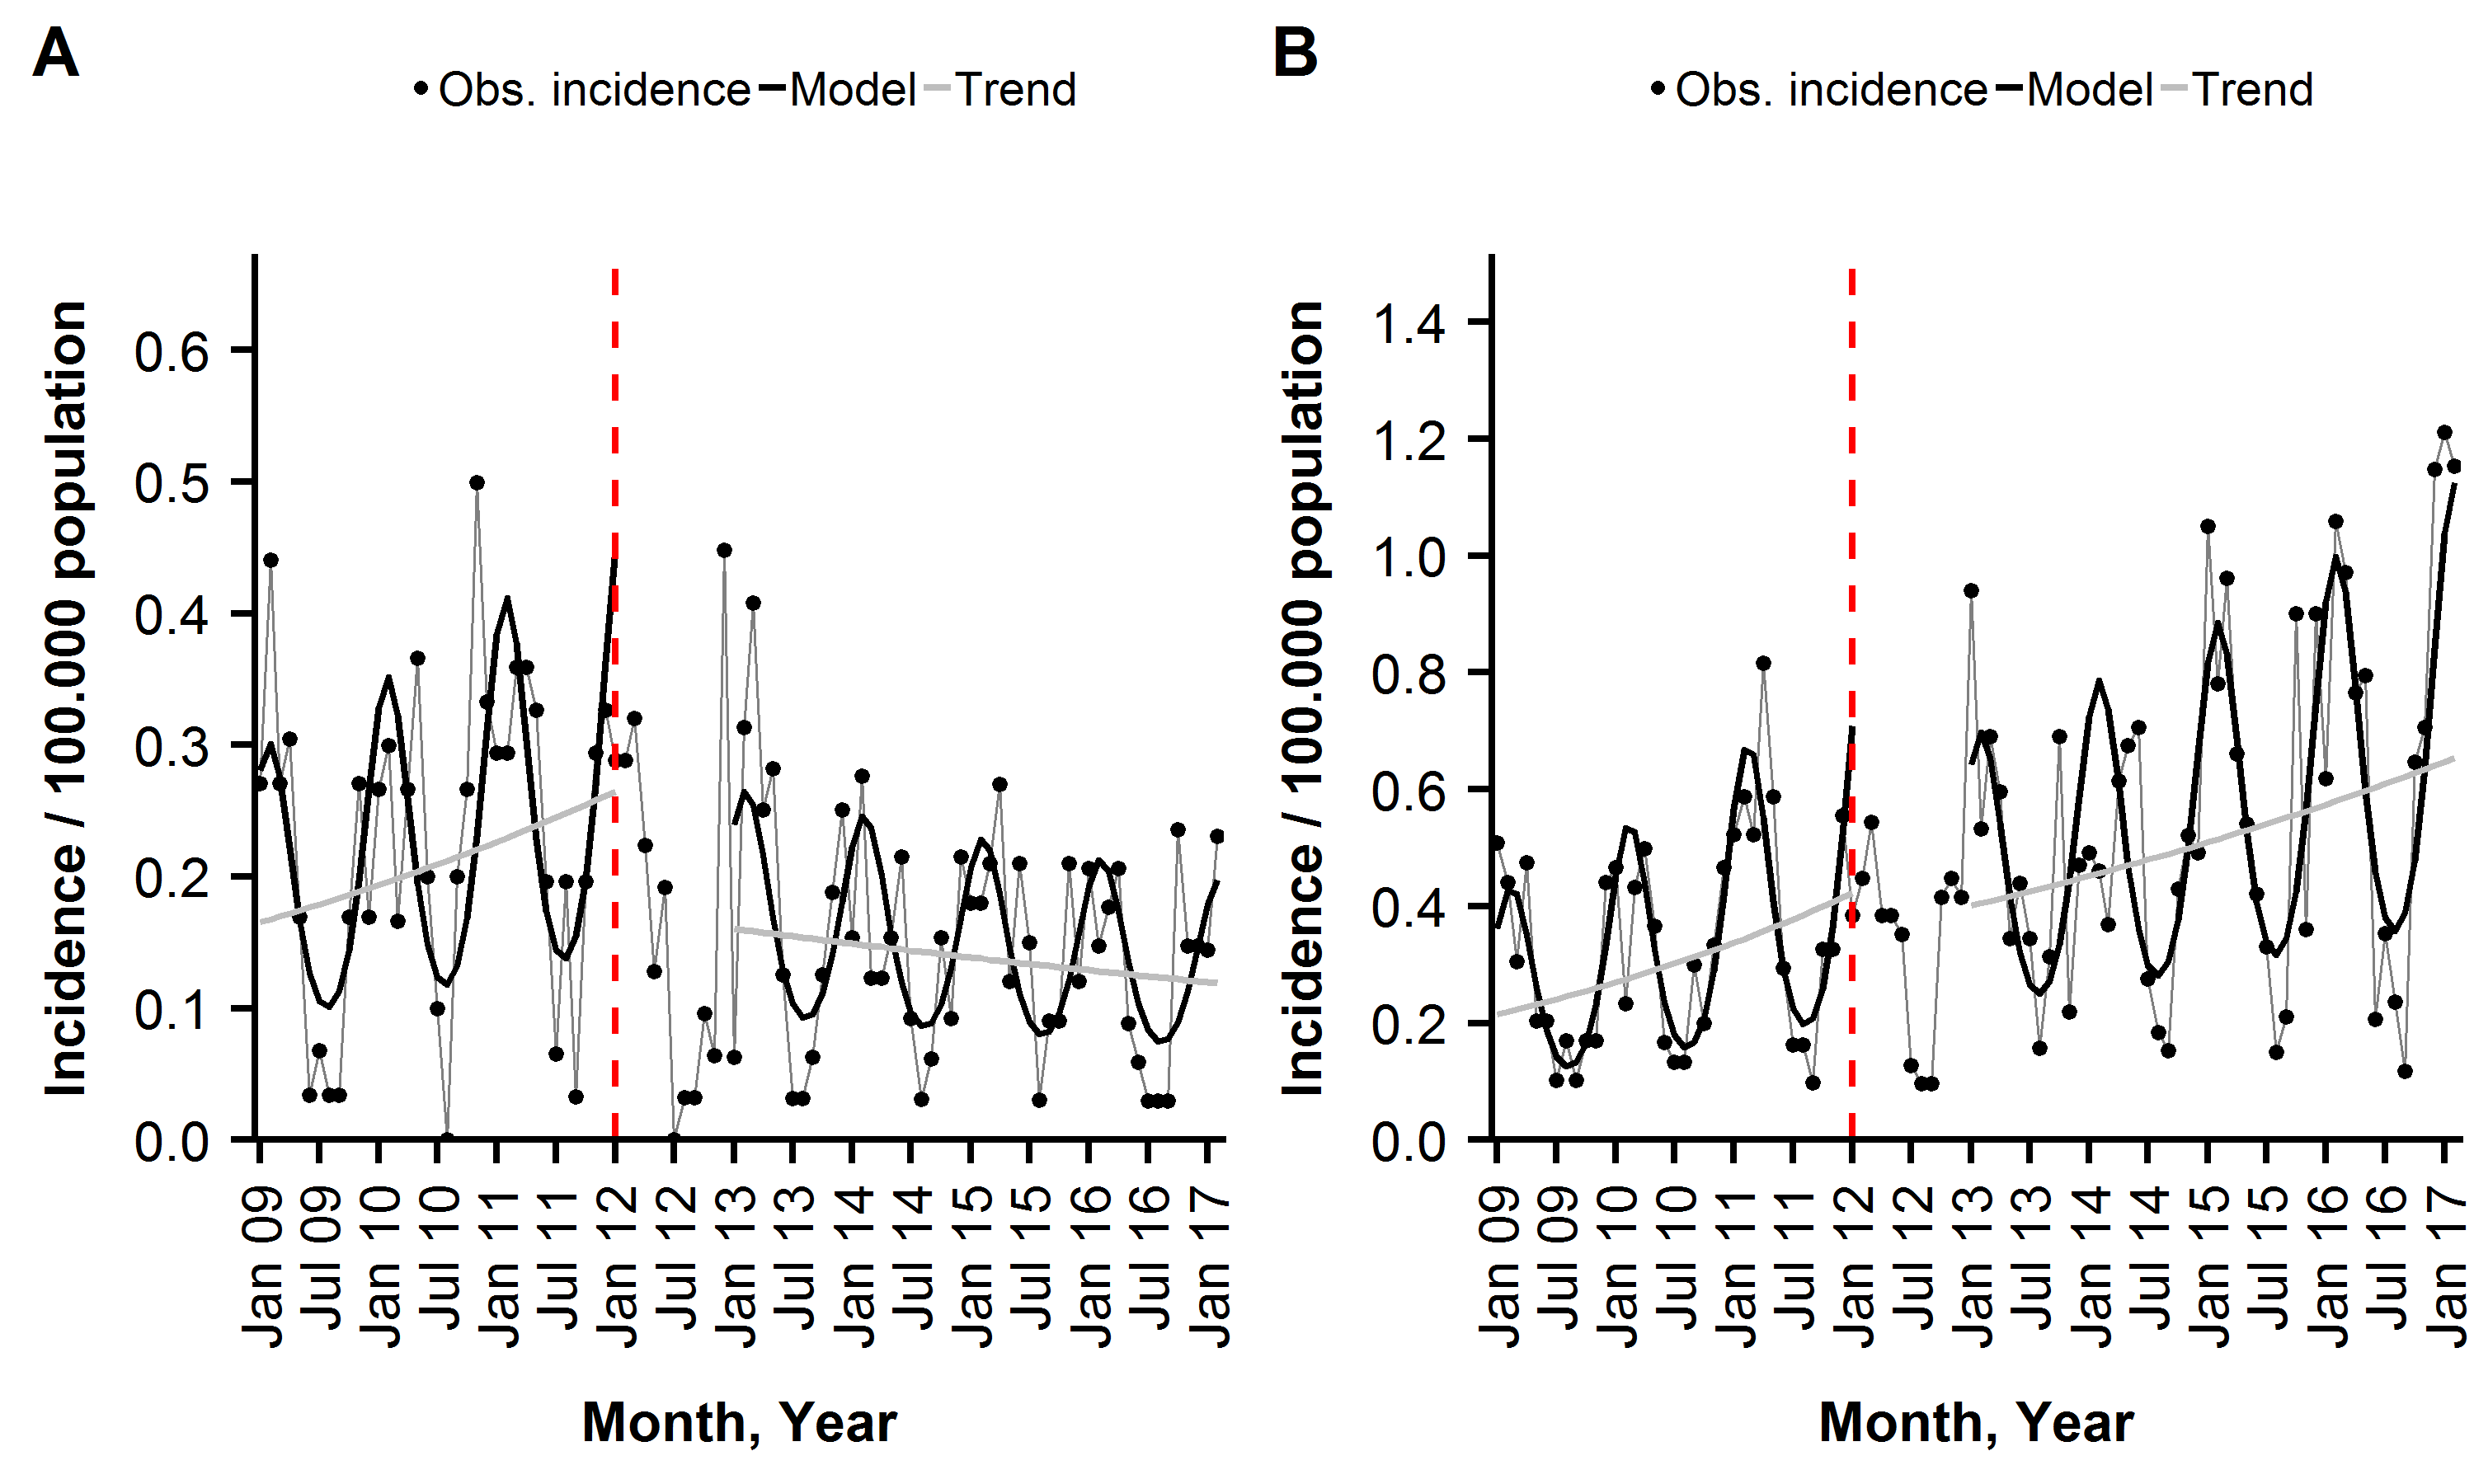
\includegraphics[width=\textwidth,height=0.5\textheight,keepaspectratio]{richter2019_Fig3.png}
\end{figure}
\end{center}
% \vfill
% {\scriptsize \cite{richter2019}}
\end{frame}
%%%%%%%%%%%%%%%%%%%%%%%%%%%%%%%%%%%%%%%%%%%%%%

\section{Dynamic models}

%%%%%%%%%%%%%%%%%%%%%%%%%%%%%%%%%%%%%%%%%%%%%%
\begin{frame}[fragile]{Mathematical modelling - Zika Virus} % source: https://www.reconlearn.org/post/practical-vbd.html

Zika introduction

\end{frame}
%%%%%%%%%%%%%%%%%%%%%%%%%%%%%%%%%%%%%%%%%%%%%%

%%%%%%%%%%%%%%%%%%%%%%%%%%%%%%%%%%%%%%%%%%%%%%
\begin{frame}[fragile]{Transmission model of Zika Virus} % source: https://www.reconlearn.org/post/practical-vbd.html

\begin{minipage}{.45\textwidth}
\rowcolors{2}{gray!8}{gray!20}
\begin{table}[]
\begin{tabular}{ll}
\hline
\rowcolor{gray!50}
Vars     & Description                                                                                          \\ \hline
$S_h$    & Susceptible Humans                                                                                   \\
$I_h$    & \begin{tabular}[c]{@{}l@{}}Infected/Infectious\\ humans\end{tabular}                                 \\
$R_h$    & \begin{tabular}[c]{@{}l@{}}Humans recovered from\\ infection (with lifelong\\ immunity)\end{tabular} \\
$S_v$    & Susceptible vectors                                                                                  \\
$E_v$    & Exposed vectors                                                                                      \\ \hline
\end{tabular}
\end{table}

\end{minipage}
\hfill
\begin{minipage}{.52\textwidth}
\vspace{1.5cm}
\begin{figure}
  \hfill 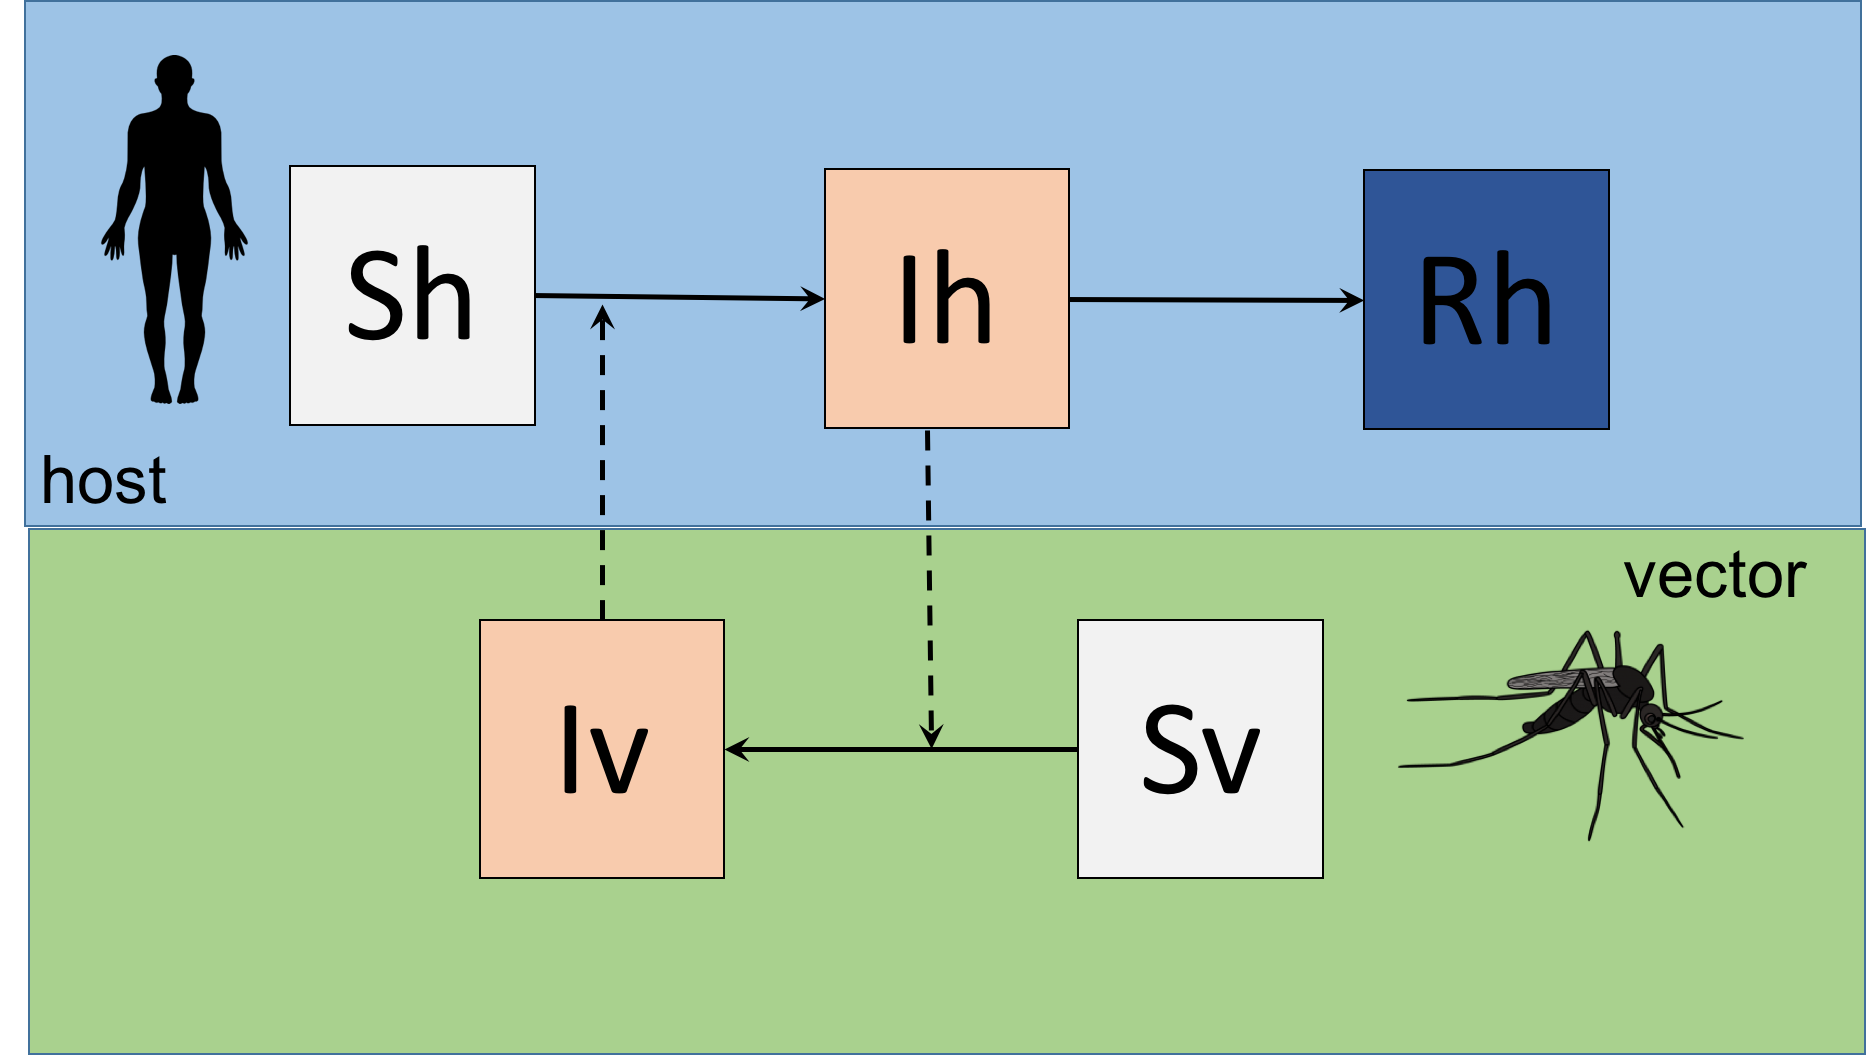
\includegraphics[width=\textwidth,height=\textheight,keepaspectratio]{SImodel.png}
\end{figure}
\vspace{1cm} {\raggedright\tiny adapted from\\ \url{https://www.reconlearn.org/} and ~\cite{ferguson2016} \par}
\end{minipage}

\end{frame}
%%%%%%%%%%%%%%%%%%%%%%%%%%%%%%%%%%%%%%%%%%%%%%

%%%%%%%%%%%%%%%%%%%%%%%%%%%%%%%%%%%%%%%%%%%%%%
\begin{frame}[fragile]{Transmission model of Zika Virus} % source: https://www.reconlearn.org/post/practical-vbd.html

\begin{minipage}{.45\textwidth}
\definecolor{my_blue}{rgb}{0.616, 0.765, 0.902}
\begin{variableblock}{Humans/Host}{bg=my_blue!30,fg=black}{bg=my_blue,fg=black}
\begin{align*}
\frac{dS_h}{dt} &= \mu_h N_h - \frac {\beta_h b}{N_h} S_h  I_v - \mu_h  S_h \\
\frac{dI_h}{dt} &= \frac {\beta_h b}{N_h}S_h I_v - (\gamma_h + \mu_h) I_h \\
\frac{dR_h}{dt} &= \gamma_h I_h  - \mu_h I_h
\end{align*}
\end{variableblock}
\definecolor{my_green}{rgb}{0.663, 0.82, 0.557}
\begin{variableblock}{Vectors}{bg=my_green!30,fg=black}{bg=my_green,fg=black}
\begin{align*}
\frac{dS_v}{dt} &= \mu_v N_v  - \frac{\beta_v b} {N_h} I_h S_v - \mu_v S_v \\
\frac{dI_v}{dt} &= \frac{\beta_v b} {N_h} I_h S_v - \mu_v I_v
\end{align*}
\end{variableblock}
\end{minipage}\hfill
\begin{minipage}{.52\textwidth}
\vspace{1.5cm}
\begin{figure}
  \hfill 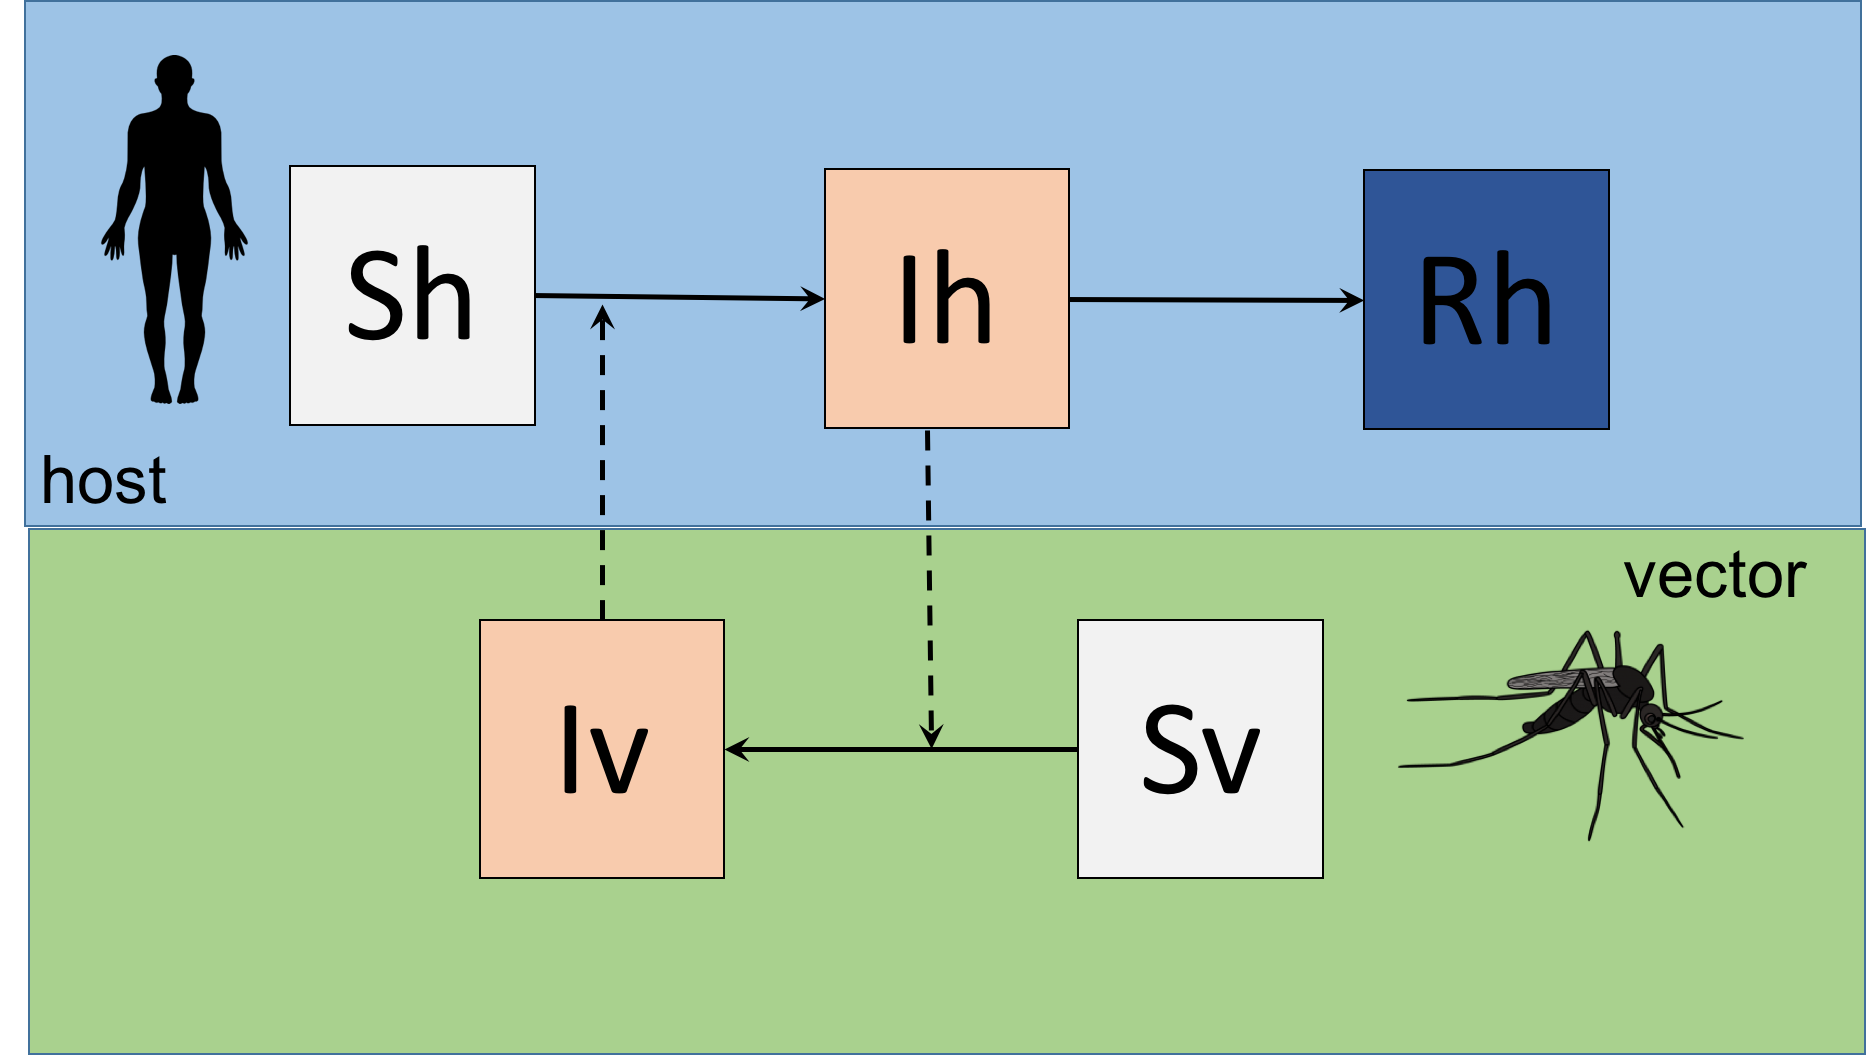
\includegraphics[width=\textwidth,height=\textheight,keepaspectratio]{SImodel.png}
\end{figure}
\vspace{1cm} {\raggedright\tiny adapted from\\ \url{https://www.reconlearn.org/} and ~\cite{ferguson2016} \par}
\end{minipage}

\end{frame}
%%%%%%%%%%%%%%%%%%%%%%%%%%%%%%%%%%%%%%%%%%%%%%


%%%%%%%%%%%%%%%%%%%%%%%%%%%%%%%%%%%%%%%%%%%%%%
\begin{frame}[fragile]{other applications}
Sexually transmitted infections \\
Ebola \\
Malaria \\

Influenza (Nielsen) \cite{nielsen2019} \\
Foodborne outbreaks to identify the source of infection (poisson model)

\end{frame}
%%%%%%%%%%%%%%%%%%%%%%%%%%%%%%%%%%%%%%%%%%%%%%

\section{Conclusion}
%%%%%%%%%%%%%%%%%%%%%%%%%%%%%%%%%%%%%%%%%%%%%%
\begin{frame}[fragile]{Conclusion/Wrap up}



We saw some examples of applied modelling\\
plays an increasingly important role in helping to guide the most high impact and cost-effective prevent disease\\
models can be critical tools in guiding public health action.\\


always comes with limitations (as other studies)\\
decision makers benefit, so do the affected people
still a lot to do - However, there are a number of challenges in achieving a successful interface between modelling and public health.


\end{frame}
%%%%%%%%%%%%%%%%%%%%%%%%%%%%%%%%%%%%%%%%%%%%%%


%%%%%%%%%%%%%%%%%%%%%%%%%%%%%%%%%%%%%%%%%%%%%%
{\unnumbered
\begin{frame}[noframenumbering]{}
\begin{center}
\begin{figure}
  \centering
  
\includegraphics[width=\textwidth,height=0.5\textheight,keepaspectratio]{Thank-you-word-cloud.jpg}
\end{figure}

\Huge{\textbf{Any questions?}}
% \begin{figure}
%   \centering
%   
\includegraphics[width=\textwidth,height=0.1\textheight,keepaspectratio]{questions.png}
% \end{figure}

\end{center}
\end{frame}}
%%%%%%%%%%%%%%%%%%%%%%%%%%%%%%%%%%%%%%%%%%%%%%

\nocite{polonsky2019}
\nocite{serfling1967}
\nocite{metcalf2015}

\renewcommand*{\bibfont}{\scriptsize}
\setbeamertemplate{bibliography item}{\insertbiblabel}

\section*{References}
%%%%%%%%%%%%%%%%%%%%%%%%%%%%%%%%%%%%%%%%%%%%%%
{\unnumbered
\begin{frame}[noframenumbering, shrink=30]{References}
  \printbibliography
\end{frame}}
%%%%%%%%%%%%%%%%%%%%%%%%%%%%%%%%%%%%%%%%%%%%%%


\end{document}


